% ----------------------------------------------------------------------------
% Author: Rayla Kurosaki
% GitHub: https://github.com/rkp1503
% ----------------------------------------------------------------------------

\section{Numerical Simulations}\label{sec:numerical_simulations}
In \myref[Section]{sec:equilibria-analysis}, we used mathematical analysis to compute the equilibria that exists in \myref[Model]{model:rayla-ephraim} and determined the conditions for stability of each one. In this section, we will support and verify the stable equilibria determined in \myref[Section]{sec:equilibria-analysis} through numerical simulations. Also, we will show the existence of a hopf bifurcation for the interior equilibrium.

\begin{figure}[H]
    \centering
    \subfloat[$z$-axial equilibrium with the set of parameters~\eqref{params:axial-z}]{%
    \resizebox*{7cm}{!}{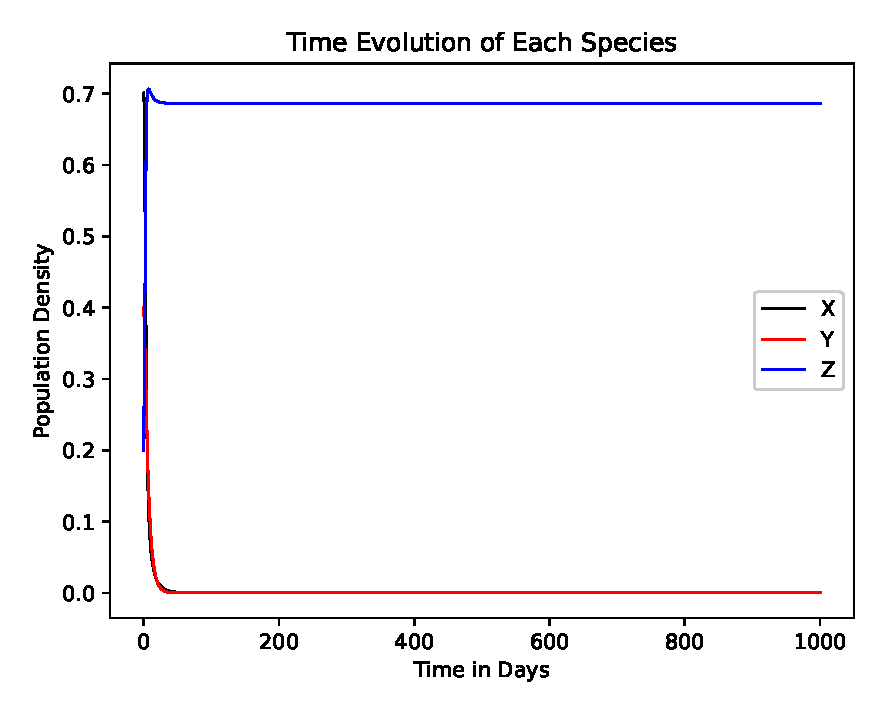
\includegraphics{equilibrium-axial-z.eps}\label{fig:axial-z}}}\hspace{5pt}
    \subfloat[$xy$-boundary equilibrium with the set of parameters~\eqref{params:boundary-xy}]{%
    \resizebox*{7cm}{!}{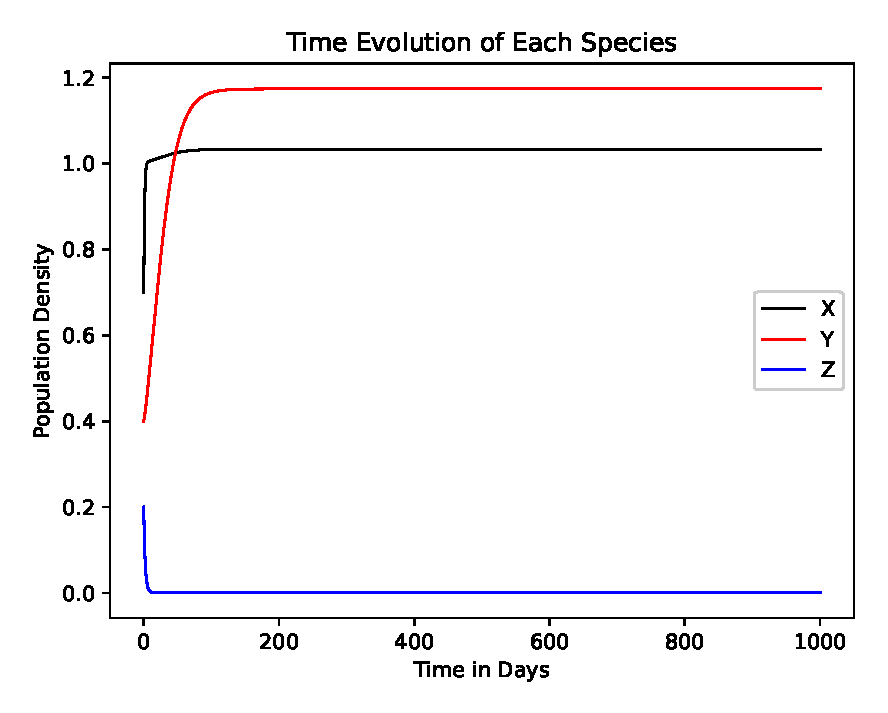
\includegraphics{equilibrium-boundary-xy.eps}\label{fig:boundary-xy}}}\hspace{5pt}
    \subfloat[$xz$-boundary equilibrium with the set of parameters~\eqref{params:boundary-xz}]{%
    \resizebox*{7cm}{!}{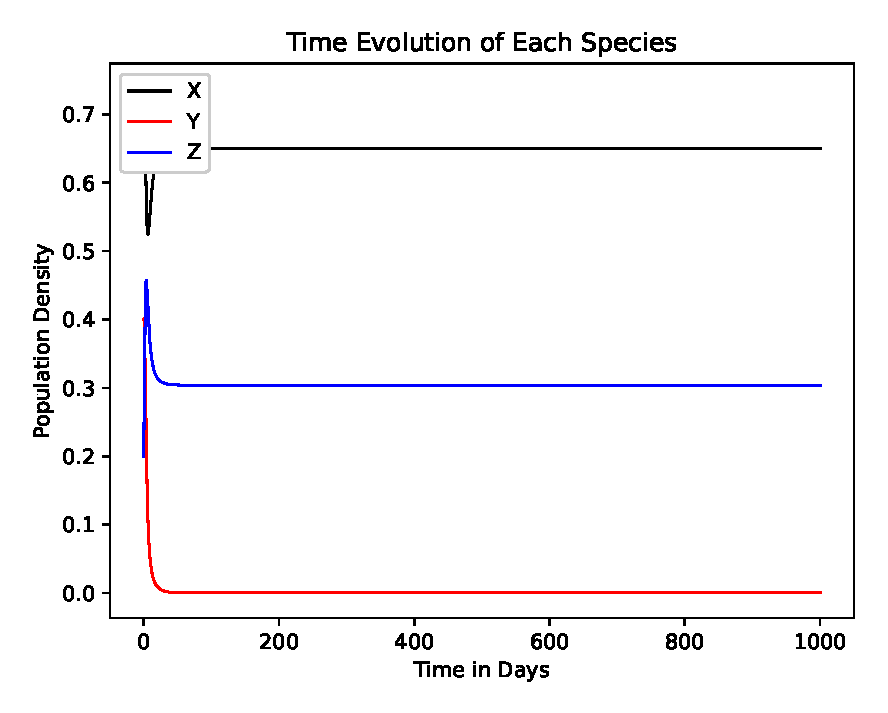
\includegraphics{equilibrium-boundary-xz.eps}\label{fig:boundary-xz}}}\hspace{5pt}
    \subfloat[$yz$-boundary equilibrium with the set of parameters~\eqref{params:boundary-yz}]{%
    \resizebox*{7cm}{!}{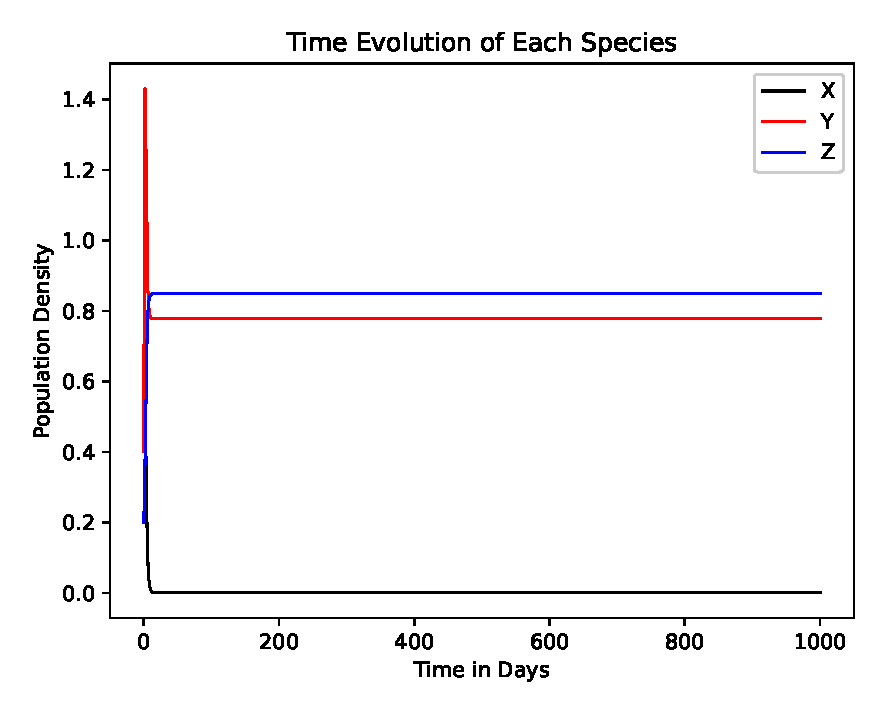
\includegraphics{equilibrium-boundary-yz.eps}\label{fig:boundary-yz}}}
    \caption{Showing the stability of non-interior equilibria for different set of parameters.}
    \label{fig:semi-trivial-equilibria-plots}
\end{figure}

\subsection{The $z$-axial equilibrium}\label{subsec:numsim_z_axial_equilibrium}
By \myref[Theorem]{thm:axial-z-exist} and \myref[Theorem]{thm:axial-z-stability}, we know that the $z$-axial equilibrium
\begin{equation*}
    E_z=\left(0,0,\frac{r_2-v_2}{\gamma_{31}r_2}\right)
\end{equation*}
exists if the condition $r_{zx} > u_4$ is satisfied and is stable if the following conditions are satisfied:
\begin{equation*}
    \frac{u_4}{r_{zx}} < 1-\frac{1}{\varphi_{xz}},\quad
    \frac{u_4}{r_{zx}} < 1-\frac{r_{yx}u_2}{u_1\left(1-p\right)},\quad
    \frac{u_4}{r_{zx}} < \frac{1}{2}
\end{equation*}
To satisfy the conditions above, lets consider the following set of parameters:
\begin{equation}\label{params:axial-z}
    \begin{dcases}
        \begin{aligned}
            r_{yx} &= 0.007\\
            r_{zx} &= 1.136\\
            p &= 0.874
        \end{aligned}
    \end{dcases},\quad 
    \begin{dcases}
        \begin{aligned}
            \varphi_{xy} &= 0.318\\
            \varphi_{yx} &= 0.416\\
            \varphi_{xz} &= 1.59
        \end{aligned}
    \end{dcases},\quad 
    \begin{dcases}
        \begin{aligned}
            u_1 &= 1.655\\
            u_2 &= 0.791\\
            u_3 &= 0.994\\
            u_4 &= 0.356
        \end{aligned}
    \end{dcases}
\end{equation}
Under this set of parameter values, the $z$-axial equilibrium is $E_z=(0,0,0.6866)$. This is further supported by \myref[Figure]{fig:axial-z}, which is the result of numerically solving \myref[Model]{model:rayla-ephraim}.

\subsection{The $xy$-boundary equilibrium}\label{subsec:numsim_xy_boundary_equilibrium}
By \myref[Theorem]{thm:boundary-xy-exist} and \myref[Theorem]{thm:boundary-xy-stability}, we know that the $xy$-boundary equilibrium $E_{xy}=\left(x^*,y^*,0\right)$ exists where $x^*=1+\varphi_{xy}\left(y^*\right)^2$ and $y^*$ is a positive solution to the equation:
\begin{equation*}
    \varphi_{xy}^2\varphi_{yx}\left(y^*\right)^4+2\varphi_{xy}\varphi_{yx}\left(y^*\right)^2-y^*+\varphi_{yx}+1=0
\end{equation*}
which can be achieved under the following condition
\begin{equation*}
    \varphi_{yx}<\frac{\beta-1}{\left(\varphi_{xy}\beta^2+1\right)^2}
\end{equation*}
for some $\beta\in\left(1, \infty\right)$ and the equilibrium is locally stable when $C_2>0,\ C_1>0,\ C_0>0,\ C_2C_1>C_0$ where:
\begin{align*}
    C_2 &= -j_{11}-j_{22}-j_{33}\\
    C_1 &= j_{11}j_{22}+j_{11}j_{33}+j_{22}j_{33}-j_{12}j_{21}\\
    C_0 &= j_{33}\left(j_{12}j_{21}-j_{11}j_{22}\right)\\
    j_{11} &= 1-2x+\varphi_{xy}\left(y^*\right)^2\\
    j_{12} &= 2\varphi_{xy}x^*y^*\\
    j_{21} &= 2r_{yx}\varphi_{yx}x^*y^*\\
    j_{22} &= r_{yx}\left(1-2y^*+\varphi_{yx}\left(x^*\right)^2\right)\\
    j_{33} &= r_{zx}+\frac{u_3\left(1-p\right)y^*}{u_2+\left(1-p\right)y^*}-u_4
\end{align*}
To satisfy the conditions above, we will let $\beta=11$ and consider the following set of parameters:
\begin{equation}\label{params:boundary-xy}
    \begin{dcases}
        \begin{aligned}
            r_{yx} &= 0.049\\
            r_{zx} &= 0.467\\
            p &= 0.645
        \end{aligned}
    \end{dcases},\quad 
    \begin{dcases}
        \begin{aligned}
            \varphi_{xy} &= 0.024\\
            \varphi_{yx} &= 0.163\\
            \varphi_{xz} &= 0.031
        \end{aligned}
    \end{dcases},\quad
    \begin{dcases}
        \begin{aligned}
            u_1 &= 0.31\\
            u_2 &= 0.978\\
            u_3 &= 0.9\\
            u_4 &= 1.004
        \end{aligned}
    \end{dcases}
\end{equation}
Under this set of parameter values, the $xy$-boundary equilibrium is $E_{xy}=(1.0331,1.174,0)$. This is further supported by \myref[Figure]{fig:boundary-xy}, which is the result of numerically solving \myref[Model]{model:rayla-ephraim}.

\subsection{The $xz$-boundary equilibrium}\label{subsec:numsim_xz_boundary_equilibrium}
By \myref[Theorem]{thm:boundary-xz-exist} and \myref[Theorem]{thm:boundary-xz-stability}, we know that the $xz$-boundary equilibrium $E_{xz}=\left(x^*,\ 0,\ z^*\right)$ exist where
\begin{equation*}
    x^*=1-\varphi_{xz}\left(1-\frac{u_4}{r_{zx}}\right),\quad
    z^*=1-\frac{u_4}{r_{zx}}
\end{equation*}
provided that the conditions have been satisfied.
\begin{equation*}
    \frac{u_4}{r_{zx}}+\frac{1}{\varphi_{xz}} > 1,\quad 
    r_{zx}>u_4
\end{equation*}
and the equilibrium is locally stable when:
\begin{equation*}
    z^*>\frac{1-2x^*}{\varphi_{xz}},\quad
    z^*>\frac{r_{yx}u_2\left(1+\varphi_{yx}\left(x^*\right)^2\right)}{u_1\left(1-p\right)},\quad
    z^*>\frac{r_{zx}-u_4}{2r_{zx}}
\end{equation*}
To satisfy the conditions above, lets consider the following set of parameters:
\begin{equation}\label{params:boundary-xz}
    \begin{dcases}
        \begin{aligned}
            r_{yx} &= 0.199\\
            r_{zx} &= 1.494\\
            p &= 0.482
        \end{aligned}
    \end{dcases},\quad 
    \begin{dcases}
        \begin{aligned}
            \varphi_{xy} &= 0.449\\
            \varphi_{yx} &= 0.993\\
            \varphi_{xz} &= 1.152
        \end{aligned}
    \end{dcases},\quad
    \begin{dcases}
        \begin{aligned}
            u_1 &= 1.671\\
            u_2 &= 0.663\\
            u_3 &= 1.556\\
            u_4 &= 1.04
        \end{aligned}
    \end{dcases}
\end{equation}
Under this set of parameter values, the $xz$-boundary equilibrium is $E_{xz}=(0.6499,0,0.3039)$. This is further supported by \myref[Figure]{fig:boundary-xz}, which is the result of numerically solving \myref[Model]{model:rayla-ephraim}.

\subsection{The $yz$-boundary equilibrium}\label{subsec:numsim_yz_boundary_equilibrium}
By \myref[Theorem]{thm:boundary-yz-exist} and \myref[Theorem]{thm:boundary-yz-stability}, we know that the $yz$-boundary equilibrium $E_{yz}=\left(0,\ y^*,\ z^*\right)$ exists where
\begin{equation*}
    z^*=1+\frac{1}{r_{zx}}\left(\frac{u_3\left(1-p\right)y^*}{u_2+\left(1-p\right)y^*}-u_4\right)
\end{equation*}
and $y^*$ is a positive solution to 
\begin{equation*}
    \frac{Y_3\left(y^*\right)^3+Y_2\left(y^*\right)^2+Y_1y^*+Y_0}{r_{zx}\left(u_2+\left(1-p\right)y^*\right)^2}=0
\end{equation*}
where:
\begin{align*}
    Y_3 &= -r_{yx}r_{zx}\left(1-p\right)^2\\
    Y_2 &= r_{yx}r_{zx}\left(1-p\right)\left(\left(1-p\right)-2u_2\right)\\
    Y_1 &= u_1\left(u_4-u_3-r_{zx}\right)\left(1-p\right)^2+r_{yx}r_{zx}u_2\left(2\left(1-p\right)-u_2\right)\\
    Y_0 &= u_2\left(r_{yx}r_{zx}u_2+u_1\left(u_4-r_2\right)\left(1-p\right)\right)
\end{align*}
provided that the following conditions are satisfied:
\begin{equation*}
    y^* > \frac{u_2\left(u_4-r_{zx}\right)}{\left(u_3-u_4+r_{zx}\right)\left(1-p\right)},\quad 
    1 > \frac{u_1\left(r_2-u_4\right)\left(1-p\right)}{r_{yx}r_{zx}u_2}
\end{equation*}
and the equilibrium is locally stable when $C_2>0,\ C_1>0,\ C_0>0,\ C_2C_1>C_0$ where:
\begin{align*}
    C_2 &= -j_{11}-j_{22}-j_{33}\\
    C_1 &= j_{11}j_{22}+j_{11}j_{33}+j_{22}j_{33}-j_{23}j_{32}\\
    C_0 &= j_{11}\left(j_{23}j_{32}-j_{22}j_{33}\right)\\
    j_{11} &= 1+\varphi_{xy}\left(y^*\right)^2-\varphi_{xz}z^*\\
    j_{22} &= r_{yx}\left(1-2y^*\right)-\frac{u_1u_2\left(1-p\right)z^*}{\left(u_2+\left(1-p\right)y^*\right)^2}\\
    j_{23} &= -\frac{u_1\left(1-p\right)y^*}{u_2+\left(1-p\right)y^*}\\
    j_{32} &= \frac{u_2u_3\left(1-p\right)z^*}{\left(u_2+\left(1-p\right)y\right)^2}\\
    j_{33} &= r_{zx}\left(1-2z^*\right)+\frac{u_3\left(1-p\right)y^*}{u_2+\left(1-p\right)y^*}-u_4
\end{align*}
To satisfy the conditions above, lets consider the following set of parameters:
\begin{equation}\label{params:boundary-yz}
    \begin{dcases}
        \begin{aligned}
            r_{yx} &= 1.219\\
            r_{zx} &= 0.452\\
            p &= 0.589
        \end{aligned}
    \end{dcases},\quad 
    \begin{dcases}
        \begin{aligned}
            \varphi_{xy} &= 0.047\\
            \varphi_{yx} &= 1.587\\
            \varphi_{xz} &= 1.908
        \end{aligned}
    \end{dcases},\quad
    \begin{dcases}
        \begin{aligned}
            u_1 &= 1.658\\
            u_2 &= 1.812\\
            u_3 &= 1.473\\
            u_4 &= 0.289
        \end{aligned}
    \end{dcases}
\end{equation}
Under this set of parameter values, the $yz$-boundary equilibrium is $E_{yz}=(0,0.7773,0.8491)$. This is further supported by \myref[Figure]{fig:boundary-yz}, which is the result of numerically solving \myref[Model]{model:rayla-ephraim}.

\subsection{The interior equilibrium}\label{subsec:numsim_interior_equilibrium}
By \myref[Theorem]{thm:boundary-yz-exist} and \myref[Theorem]{thm:boundary-yz-stability}, we know that the interior equilibrium $E_{xyz}=\left(x^*,\ y^*,\ z^*\right)$ exists where
\begin{equation*}
    x^*=1+\varphi_{xy}\left(y^*\right)^2-\varphi_{xz}z^*,\quad 
    z^*=1+\frac{1}{r_{zx}}\left(\frac{u_3\left(1-p\right)y^*}{u_2+\left(1-p\right)y^*}-u_4\right)
\end{equation*}
and $y^*$ is a positive solution to 
\begin{equation*}
    \frac{Y_6\left(y^*\right)^6+Y_5\left(y^*\right)^5+Y_4\left(y^*\right)^4+Y_3\left(y^*\right)^3+Y_2\left(y^*\right)^2+Y_1y^*+Y_0}{r_{zx}^2\left(u_2+\left(1-p\right)y^*\right)^3}=0
\end{equation*}
where:
\begin{align*}
    Y_6 &= r_{yx}r_{zx}^2\varphi_{xy}^2\varphi_{yx}\left(1-p\right)^2\\
    Y_5 &= 2r_{yx}r_{zx}^2u_2\varphi_{xy}^2\varphi_{yx}\left(1-p\right)\\
    Y_4 &= r_{yx}r_{zx}\varphi_{xy}\varphi_{yx}\left(2\left(r_{zx}\left(1-\varphi_{xz}\right)+\varphi_{xz}\left(u_4-u_3\right)\right)\left(1-p\right)^2+r_{zx}u_2^2\varphi_{xy}\right)\\
    Y_3 &= r_{yx}r_{zx}\left(1-p\right)\left(-r_{zx}\left(1-p\right)+2u_2\varphi_{xy}\varphi_{yx}\left(2r_{zx}\left(1-\varphi_{xz}\right)+\varphi_{xz}\left(2u_4-u_3\right)\right)\right)\\
    Y_2 &= r_{yx}\left(\left(\varphi_{yx}\left(r_{zx}\left(1-\varphi_{xz}\right)+\varphi_{xz}\left(u_4-u_3\right)\right)^2+r_{zx}^2\right)\left(1-p\right)^2-2r_{zx}^2u_2\left(1-p\right)\right.\\
    &\left.+2r_{zx}\varphi_{xy}\varphi_{yx}u_2^2\left(r_{zx}\left(1-\varphi_{xz}\right)+u_4\varphi_{xz}\right)\right)\\
    Y_1 &= r_{zx}u_1\left(u_4-u_3-r_{zx}\right)\left(1-p\right)^2+2r_{yx}u_2\left(r_{zx}^2\left(\varphi_{yx}\left(\varphi_{xz}-1\right)^2+1\right)\right.\\
    &\left.+\varphi_{xz}\varphi_{yx}\left(-u_4\left(2r_{zx}\left(\varphi_{xz}-1\right)+\varphi_{xz}u_3\right)+r_{zx}u_3\left(\varphi_{xz}-1\right)+\varphi_{xz}u_4^2\right)\right)\left(1-p\right)\\
    &-r_{yx}r_{zx}^2u_2^2\\
    Y_0 &= u_2\left(r_{zx}u_1\left(u_4-r_{zx}\right)\left(1-p\right)+r_{yx}u_2\left(\varphi_{yx}\left(\varphi_{xz}\left(r_{zx}-u_4\right)-r_{zx}\right)^2+r_{zx}^2\right)\right)
\end{align*}
provided that the following conditions are satisfied:
\begin{equation*}
    \frac{1+\varphi_{xy}\left(y^*\right)^2}{\varphi_{xz}}>z^*,\quad
    y^*>\frac{u_2\left(u_4-r_{zx}\right)}{\left(u_3-\left(u_4-r_{zx}\right)\right)\left(1-p\right)},\quad
    Y_0 < 0
\end{equation*}
and the equilibrium is locally stable when $C_2>0,\ C_1>0,\ C_0>0,\ C_2C_1>C_0$ where:
\begin{align*}
    C_2 &= -j_{11}-j_{22}-j_{33}\\
    C_1 &= j_{11}j_{22}+j_{11}j_{33}+j_{22}j_{33}-j_{12}j_{21}-j_{23}j_{32}\\
    C_0 &= j_{11}\left(j_{23}j_{32}-j_{22}j_{33}\right)+j_{21}\left(j_{12}j_{33}-j_{13}j_{32}\right)\\
    j_{11} &= 1-2x^*+\varphi_{xy}\left(y^*\right)^2-\varphi_{xz}z^*\\
    j_{12} &= 2\varphi_{xy}x^*y^*\\
    j_{13} &= -\varphi_{xz}x^*\\
    j_{21} &= 2r_{yx}\varphi_{yx}x^*y^*\\
    j_{22} &= r_{yx}\left(1-2y^*+\varphi_{yx}\left(x^*\right)^2\right)-\frac{u_1u_2\left(1-p\right)z^*}{\left(u_2+\left(1-p\right)y^*\right)^2}\\
    j_{23} &= -\frac{u_1\left(1-p\right)y^*}{u_2+\left(1-p\right)y^*}\\
    j_{32} &= \frac{u_2u_3\left(1-p\right)z^*}{\left(u_2+\left(1-p\right)y^*\right)^2}\\
    j_{33} &= r_{zx}\left(1-2z^*\right)+\frac{u_3\left(1-p\right)y^*}{u_2+\left(1-p\right)y^*}-u_4
\end{align*}
To ensure that the interior equilibrium exist and is stable, lets consider the following set of parameters:
\begin{equation}\label{params:interior-a}
    \begin{dcases}
        \begin{aligned}
            r_{yx} &= 0.5\\
            r_{zx} &= 0.5\\
            p &= 0.6
        \end{aligned}
    \end{dcases},\quad 
    \begin{dcases}
        \begin{aligned}
            \varphi_{xy} &= 0.6\\
            \varphi_{yx} &= 0.15\\
            \varphi_{xz} &= 0.4
        \end{aligned}
    \end{dcases},\quad
    \begin{dcases}
        \begin{aligned}
            u_1 &= 0.6\\
            u_2 &= 0.08\\
            u_3 &= 0.5\\
            u_4 &= 0.5
        \end{aligned}
    \end{dcases}
\end{equation}
Under this set of parameter values, the interior equilibrium is $E_{xyz}=(0.9099,0.0599,0.2305)$. This is further supported by the four figures in \myref[Figure]{fig:nontrivial-equilibria-plots} where \myref[Figure]{fig:time-evolution} shows the time evolution of each Species, \myref[Figure]{fig:phase-plane-3d} shows the phase portrait, and \myref[Figure]{fig:phase-plane-xy}, \myref[Figure]{fig:phase-plane-xz}, and \myref[Figure]{fig:phase-plane-yz} are phase planes when numerically solving \myref[Model]{model:rayla-ephraim}.

For \myref[Model]{model:rayla-ephraim}, we can numerically show that a hopf bifurcation exists for each parameter. Starting with $r_{zx}$, we will plot the time evolution of the ecosystem at $r_{zx}=0.35$ to show that the ecosystem expresses an oscillatory behavior as shown in \myref[Figure]{fig:bifurcation-r_zx-xyz}. Then, we will generate a bifurcation diagram for Species $X,\ Y,\ Z$ over a set interval of $r_{zx}$, expressed in \myref[Figure]{fig:bifurcation-r_zx-x}, \myref[Figure]{fig:bifurcation-r_zx-y}, \myref[Figure]{fig:bifurcation-r_zx-z} respectively. For $r_{zx}$, the interval is $r_{zx}\in(0.133,0.6155)$. From the bifurcation diagrams, we can see that the ecosystem undergoes 2 changes. Denoting the stable solutions for Species $X,\ Y,\ Z$ in black, red, and blue respectively and denoting the unstable solutions in green, we can see that the ecosystem starts off in a stable state and then becomes unstable when $r_{zx}\approx 0.29$. From here, this behavior is maintained until $r_{zx}\approx 0.47$ where it transitions back to a stable state. Thus, we can say that for the set of \myref[parameters]{params:interior-a}, the ecosystem maintains a stable equilibrium when $r_{zx}\in(0.29,0.47)$ and displays an oscillatory behavior when $r_{zx}\in(0.133,0.29)$ and $r_{zx}\in(0.47,0.6155)$.
% If $r_{zx}>0.6155$, then Species $y$ dies out, turning the interior equilibrium to a $xz$-boundary equilibrium. If $r_{zx}<0.133$, then....

We can repeat this process using the same set of parameters to show that a hopf bifurcation exists for $p$, $\varphi_{yx}$, and $u_2$. For $p$, the ecosystem undergoes a hopf bifurcation at $p\approx 0.371$, shown in \myref[Figure]{fig:bifurcation-p}. For $\varphi_{yx}$, the ecosystem undergoes a hopf bifurcation at $p\approx 0.387$, shown in \myref[Figure]{fig:bifurcation-phi_yx}. For $u_2$, the ecosystem undergoes a hopf bifurcation at $u_2\approx 0.051$, shown in \myref[Figure]{fig:bifurcation-u_2}. For the other parameters $r_{yx},\ \varphi_{xy},\ \varphi_{xz},\ u_1,\ u_3,\ u_4$, we will consider the set of \myref[parameters]{params:interior-b}. Applying the above procedure to these parameters, we can conclude that the ecosystem undergoes a hopf bifurcation at $r_{yx}\approx 0.66,\ \varphi_{xy}\approx 0.125,\ \varphi_{xz}\approx\{0.402,1.342\},\ u_1\approx 0.728,\ u_3\approx\{0.511,2.501\},\ u_4\approx\{0.122,0.314\}$, depicted in \myref[Figure]{fig:bifurcation-r_yx}, \myref[Figure]{fig:bifurcation-phi_xz}, \myref[Figure]{fig:bifurcation-u_1}, \myref[Figure]{fig:bifurcation-u_3}, \myref[Figure]{fig:bifurcation-u_4} respectively.
\begin{equation}\label{params:interior-b}
    \begin{dcases}
        \begin{aligned}
            r_{yx} &= 0.5\\
            r_{zx} &= 0.5\\
            p &= 0.6
        \end{aligned}
    \end{dcases},\quad 
    \begin{dcases}
        \begin{aligned}
            \varphi_{xy} &= 0.6\\
            \varphi_{yx} &= 0.15\\
            \varphi_{xz} &= 0.4
        \end{aligned}
    \end{dcases},\quad
    \begin{dcases}
        \begin{aligned}
            u_1 &= 0.6\\
            u_2 &= 0.08\\
            u_3 &= 0.5\\
            u_4 &= 0.5
        \end{aligned}
    \end{dcases}
\end{equation}
